%% This is an example first chapter.  You should put chapter/appendix that you
%% write into a separate file, and add a line \include{yourfilename} to
%% main.tex, where `yourfilename.tex' is the name of the chapter/appendix file.
%% You can process specific files by typing their names in at the 
%% \files=
%% prompt when you run the file main.tex through LaTeX.

%\providecommand{\phasezero}{Phase-0\xspace}
%\providecommand{\phaseone}{Phase-I\xspace}
%\providecommand{\phasetwo}{Phase-II\xspace}

\providecommand{\phasezero}{Phase-0 }
\providecommand{\phaseone}{Phase-I }
\providecommand{\phasetwo}{Phase-II }

\chapter{Higgs Pair Production at the HL-LHC}

The discovery of a Higgs boson opens a new era in particle physics, the era of precision Higgs studies. The LHC is expected to undergo major updates resulting in a significant increase in the instantaneous luminosity~\cite{Apollinari:2116337}.  The injector chains will be upgraded to provide high intensity and low emittance bunches. The quadrupole magnets that focus the beam at the ATLAS and CMS interaction regions will also be upgraded along with additions of crab cavities to improve the bunch overlap at the interaction regions. These upgrades will allow proton-proton collisions with a peak instantaneous luminosity of $2\times10^{35}$ cm$^2$ s$^{-1}$. This high luminosity operation period is known as the \phasetwo or HL-LHC. 

A total integrated luminosity of about $3000~\ifb$ in proton-proton collisions at $\sqrt{s}=14~\TeV$ is expected by the end of $2035$. This large dataset will allow to make precise measurements of the Higgs boson couplings and search for its rare SM as well as BSM decays. The discovered boson has so far shown a consistent picture with the SM Higgs boson as discussed in Section 1.1. Figure~\ref{fig:coupling} shows the current CMS Higgs boson coupling measurements (left) and the projected measurements of the couplings using the HL-LHC dataset (right) as a function of the the corresponding boson and fermion masses.      
\begin{figure}[hbtp]
  \begin{center}
    \includegraphics[width=0.49\textwidth]{figures_chapter6/current}
    \includegraphics[width=0.49\textwidth]{figures_chapter6/future}       
    \caption{The SM Higgs boson couplings measured at the LHC Run $1$ data taking period (left) and the projected measurements to $3000~\ifb$ expected luminosity at the HL-LHC (right) as a function of the corresponding boson and fermion masses~\cite{Butler:2020886}.}
    \label{fig:coupling}
  \end{center}
\end{figure}
A percent level measurement can be performed for the majority of the Higgs couplings. In addition, the Higgs coupling to the second generation fermions will be accessible via the Higgs boson decays to the muon pair final state. 

It is also possible to study the SM Higgs boson trilinear coupling by considering the Higgs pair production as discussed in Section 1.4. This chapter describes the studies of the Higgs boson pair production at the HL-LHC in $bb\gamma\gamma$ and $bb\tau\tau$ final states with the upgraded CMS detector~\cite{CMS-PAS-FTR-15-002}. The gluon fusion production cross section for the Higgs boson pair production at a center of mass energy of $14$~TeV has been calculated to next-to-next-to-leading-order to be $40.7$~fb~\cite{Dawson:1998py,Grigo:2014jma}. Other production modes potentially add another $10\%$ to the total production cross section, but have not been included in this study. Approximately $320$ and  $9000$ signal events are expected to be produced per experiment at the HL-LHC for the $bb\gamma\gamma$ and $bb\tau\tau$ final states respectively.

\section{CMS \phasetwo Detector and Simulation}

The increased instantaneous luminosity leads to a significant increase in the number of additional pileup interactions. The HL-LHC is expected to operate with an average of $140$ pileup events per bunch crossing. This presents a serious challenge to the experiments in their ability to deal with this increased level of activity and energy flow, and to preserve the detector performance under this environment.  As part of a comprehensive strategy to address these issues, CMS has released a technical proposal for the \phasetwo upgrade~\cite{Butler:2020886} program. The expected performance of this detector at the HL-LHC is assumed for these studies and is discussed in the following sections. The impact of some of the individual components of the \phasetwo upgrade on the results are highlighted where it is appropriate. In addition, the $bb\gamma\gamma$ results are also described assuming the detector performance of the so called \phaseone CMS upgrade~\cite{Collaboration:1355706} detector after an assumed integrated luminosity of $1000$~$\mathrm{fb}^{-1}$; configuration hereafter denoted as ``\phaseone aged''.

At present, the \phasetwo detector simulation includes the upgraded outer tracker, muon systems, and calorimetry. The inner pixel detector upgrade, however, is still not finalized and the simulation contains the \phaseone pixel detector in the barrel and an extended version of the current pixel detector in the forward detector to provide an ability of tracking at higher $|\eta|$ values of up to $4.0$. The primary and secondary vertex reconstruction and identification performance will certainly be better than what is assumed in these studies and should be viewed as a conservative estimate.

It is crucial that the \phasetwo detector can cope with the challenging environment at the HL-LHC as pileup mitigation, b-tagging, tau reconstruction and identification, photon identification efficiencies, and mass  resolutions are fundamental to perform these measurements. Triggers are assumed to be $100\%$ efficient in these studies. The \textsc{Delphes} fast simulation framework~\cite{deFavereau:2013fsa} can be used to model the \phasetwo detector response. The parameterized response of the \phasetwo detector in Delphes is taken from the corresponding GEANT4 based fully simulated samples. The $bb\gamma\gamma$ analysis uses the MC generator truth information with smearing functions to model the response of the detector. A combination of the two approaches mentioned above is used for the $bb\tau\tau$ final state.  

The signal samples are generated using the MadGraph5\_aMC@NLO generator with LO accuracy in QCD, using the results from~\cite{Frederix2014142}. PYTHIA 6 is used to model the parton showering and hadronization. The generator is also interfaced with TAUOLA for the simulation of the tau lepton decays. The pileup events are simulated in the Delphes samples by randomly placing minimum-bias interactions along the beam axis according to the longitudinal spread of the minimum-bias interactions derived from the fully simulated samples.

\section{$bb\gamma\gamma$ Final State}

The signal events of interest contain two high transverse momentum $p_{T}$ photon candidates and two high $p_{T}$ jets originating from b quarks. The photons are rejected if an electron is reconstructed within a distance $\Delta R$ of $0.1$ to the photon.  A $p_{T}$ and $\eta$ dependent efficiency is applied to the photons to model the identification and isolation efficiency. The efficiency is about $80\%$ in the barrel, and about $55\%$ in the endcap. The lower efficiency in the endcap is primarily due to the electron veto requirement.  The jets are reconstructed using the anti-kt algorithm with a resolution parameter of $0.5$. The processes involving jets faking photons are among the dominant backgrounds. The rate to misidentify photons is about $1 \times 10^{-4}$ for gluon jets and about $5\times 10^{-4}$ for quark jets. The rate to misidentify electrons as photons is taken to be $1\%$ ($3\%$) in the barrel (endcap). Di-photon mass width of $1.2$~GeV is achieved with the upgraded detector, for the events where both photons are in the barrel, using sophisticated multivariate techniques to calibrate the photon energy.  Jets are tagged as originating from a b quark on the basis of the presence of secondary vertices and large impact parameter tracks, which are exploited for b-tagging in the CSV discriminator as discussed in Section 3.5.3. The chosen working point of the CSV discriminator gives, on average, b-tagging efficiencies of about $75\%$ and $65\%$ in the central and forward regions, respectively; with mistagging rates for light and charm jets of about $1\%$ and $20\%$, respectively. Di-jet mass resolution of about $20$~GeV is achieved with the upgraded detector. 

Electrons and muon candidates with $p_{T}>10$~GeV are selected for the purpose of vetoing events with signatures consistent with a Higgs boson produced in association with a top and anti top quark pair ($t\bar{t}H$). This process contributes significantly to the total background after signal event selection requirements. A non-negligible fraction of such background events contain leptons and can be rejected on this basis. Very loose selection requirements with efficiency in the range between $90\%$ and $95\%$ are placed on the electron and muon candidates in order to suppress this background as much as possible.

\subsection{Signal and Background Estimation}
\label{sec:bkgestimation}
The signal process of interest is the production of two Higgs bosons, one of which decays to a pair of b quarks, and the other decaying to a pair of photons. The main resonant backgrounds are $ZH$, where a Higgs boson is produced in association with a Z boson which subsequently decays to two b-jets, $t\bar{t}H$, where a Higgs boson is produced in association with a top and anti-top quark pair, and $b\bar{b}H$, where a Higgs boson is produced in association with a b and anti-b quark pair. The non-resonant backgrounds include QCD production  of $b \bar{b} \gamma\gamma$, QCD production of $jj \gamma\gamma$ with light jets mistagged  as b-jets, QCD production of $b \bar{b} j \gamma$ and $b \bar{b} jj$ with one and two jets misidentified as photons respectively, and QCD production of four jets with two jets misidentified  as photons and two jets miss-tagged as b-jets, dominated by mistagged charm jets. 
These background processes have cross sections that are several orders of magnitude larger than the resonant backgrounds, but are suppressed
by the low rate for mistaged b-jets and misidentified photons.  It is computationally impossible to fully simulate these background events due to their large cross sections. Instead, generator particle truth level MC samples are produced and the events are weighted by the corresponding efficiencies and fake rates for selecting the constituent particles. Finally, the SM  production of $t\bar{t}(\gamma)$ enters as background for the signal event selection for events where both top quarks decay semi-leptonically to electrons where one (or both) of the electrons are misidenified as photons. A sample of di-electron decays of the $t\bar{t}(\gamma)$ events are weighted by the corresponding electron to photon misidenification rates to estimate the background contribution.

%The cross sections for the non-resonant background processes are summarized in Table~\ref{tab:CrossSections}. Recent studies of the non-resonant background production of the $b \bar{b} \gamma\gamma$ show that the rate is significantly enhanced (by a factor of about two) when full NLO simulation is performed~\cite{Azatov:2015oxa}. The NLO simulation includes both the real and virtual corrections. 

%\begin{table}[!ht]
%\begin{center} 
%\begin{tabular}{|c|c|}
%\hline
%Process                                           &   Cross Section (fb)   \\ \hline
%$b \bar{b} \gamma\gamma$                          &   $272$                            \\
%$jj \gamma\gamma$                                 &   $2.2 \times 10^{4}$              \\
%$bb j\gamma$                                      &   $8.1 \times 10^{5}$              \\
%$cc j\gamma$                                      &   $2.5 \times 10^{6}$              \\
%$bb jj$                                           &   $6.1 \times 10^{8}$              \\
%$cc jj$                                           &   $6.5 \times 10^{8}$              \\
%$jjjj$                                            &   $2.0 \times 10^{10}$             \\ \hline
%\end{tabular}
%\caption{ The production cross sectiona of the non-resonant background processes at a center of mass energy 
%of $14$~TeV.}
%\label{tab:CrossSections}
%\end{center}
%\end{table}

\subsection{Event Selection}
\label{sec:eventselection}
 
Events containing two photons with $p_{T}$ greater than $25$~GeV
and $|\eta|<2.5$, and two b-tagged jets with $p_{T}$ greater than $30$~GeV and $|\eta|<2.4$ are selected. While the \phasetwo upgrades allow b-jet tagging capabilities up to $|\eta|$ of $3.0$, the b-tagged jets with $p_{T}$ greater than $30$~GeV for the signal events are predominantly central and therefore b-tagged jets with $|\eta|<2.4$ are selected. One of the two photons is required to have $p_{T} > 40$~GeV. Due to the large amount of background from jets faking photons in the endcap region of the detector the event sample is split into two categories: one with both photons in the barrel and one with at least one photon in the endcap. To suppress $t\bar{t}H$ background events, it is required that there are no electrons or muons passing the veto selection and that  the number of jets with $p_{T}>30$~GeV and $|\eta|<2.5$ is less than four. 

A number of different additional kinematic requirements were investigated in order to improve the signal to background ratio. It is required that the $\Delta R$ between the two photons and the $\Delta$R between the two b-jets are less than $2.0$, and that the minimum of the  $\Delta R$ between photons and b-jets is larger than $1.5$. With the above kinematic selection requirements, a signal to background ratio of about $1:3$ is achieved.

The expected event yields for the signal and resonant background processes, and the  non-resonant background processes for various stages of the event selection
are shown in Table~\ref{tab:EventYields}. For the event category with both photons in the barrel, the dominant backgrounds are $bb\gamma\gamma$, $jj\gamma\gamma$ primarily consisting of mistagged charm jets, and $bbj\gamma$ with one fake photon, while for the event category with at least one photon in the endcap the dominant backgrounds are $bbj\gamma$ and $bbjj$ with one or two fake photons.

\begin{table}[!ht]
\begin{center} 
\resizebox{\textwidth}{!}{
\begin{tabular}{|c|c|c|c|c|}
\hline
Process / Selection Stage            &  $HH \rightarrow b\bar{b}\gamma\gamma$  &  $ZH \rightarrow b\bar{b}\gamma\gamma$ &  $t\bar{t}H \rightarrow W W b \bar{b}\gamma\gamma$ &  $b\bar{b}H$                   \\  \hline
Object Selection \&                  &  \multirow{2}{*}{23.8 (6.27)}            &  \multirow{2}{*}{30.5 (12.0)}           &  \multirow{2}{*}{184 (47.2)}                      &  \multirow{2}{*}{6.53 (2.61)}    \\ 
Fit Mass Window                      &                                         &                                        &                                                    &                                \\ 

Kinematic Selection                  &  13.4 (3.27)                             &  15.1  (4.44)                            &  3.39  (1.04)                                        &  2.09 (0.78)       \\ 
Mass Windows                         &  9.00 (1.91)                              &  3.39  (0.26)                            &  1.57 (0.26)                                         &  0.78 (0.26)       \\  \hline
\end{tabular}
}
\vspace{2mm}
\begin{tabular}{|c|c|c|}
\hline
Process / Selection Stage           &  $b \bar{b} \gamma\gamma$   & $jj \gamma\gamma$            \\  \hline
Object Selection \&                 &  \multirow{2}{*}{2767 (1363)} & \multirow{2}{*}{954 (552)} \\ 
Fit Mass Window                     &                             &                              \\ 
Kinematic Selection                 &  162  (88.8)                 &  30.2  (19.7)                      \\ 
Mass Windows                        &  10.4 (5.70)                &  2.1 (1.2)                     \\  \hline
\end{tabular}
\vspace{2mm}
\resizebox{\textwidth}{!}{
\begin{tabular}{|c|c|c|c|c|c|}
\hline
Process / Selection Stage           &  $bb j\gamma$                  &  $ccj\gamma$                  & $bb jj$                    &  $ccjj$                       & $t\bar{t}(\gamma)$                \\  \hline
Object Selection \&                 &  \multirow{2}{*}{1592 (5145)}   &  \multirow{2}{*}{27.2 (46.3)}   & \multirow{2}{*}{279 (1622)} &  \multirow{2}{*}{7.8 (44.4)}  &  \multirow{2}{*}{597 (705)} \\ 
Fit Mass Window                     &                                &                               &                            &                               &                           \\ 
Kinematic Selection                 &  96.9  (351)                     &  0.7  (3.7)                   & 19.6 (137)                   &  0.2 (2.1)                    &  21.5 (20.3)                \\ 
Mass Windows                        &  6.3 (17.2)                     &  0.0  (0.2)                   & 1.1 (7.9)                 &  0.02 (0.1)                   &  1.2 (1.2)                \\  \hline
\end{tabular}
}
\caption{ The expected event yields of the signal and background processes
for $3000$~$\mathrm{fb}^{-1}$ of integrated luminosity at various stages of the cut-based selection for 
the category with both photons in the barrel. The event yields for the category with at least one photon in the endcap are shown inside the brackets. A large fit mass
window, $105$~GeV to $145$~GeV for $\mathrm{M}_{\gamma\gamma}$ and $70$~GeV to $200$~GeV for $\mathrm{M}_{bb}$,
is used for the likelihood fit analysis described in Section~\ref{sec:signalextraction}. }
\label{tab:EventYields}
\end{center}
\end{table}


\subsection{Signal Extraction}
\label{sec:signalextraction}

To extract the signal cross section, the kinematic selection requirements from Section~\ref{sec:eventselection} are applied, and a two dimensional maximum
likelihood fit on the di-photon and di-bjet mass distributions is performed. Probability density functions are derived for the di-photon mass, $\mathrm{M}_{\gamma\gamma}$, and di-bjet mass, $\mathrm{M}_{bb}$,
distributions for the signal, the resonant background, and the non-resonant background by 
fitting the distributions from the simulated samples to a particular parametrization 
of the line-shape for $\mathrm{M}_{\gamma\gamma}$ and $\mathrm{M}_{bb}$. The distributions of the signal and resonant backgrounds are fitted with a Crystal Ball distribution, while for
the non-resonant backgrounds are fitted to a decaying exponential. The jet energy resolution parameter is then appropriately increased to model the degraded jet energy resolution under the HL-LHC pileup conditions,

The correlations between $\mathrm{M}_{\gamma\gamma}$ and $\mathrm{M}_{bb}$ are assumed to be negligible. Therefore, the two dimensional probability distribution functions are simply the product of the one dimensional probability distribution functions. The expected number of events within the fit mass window is used to normalize the probability distributions functions for the signal, the resonant background, and the non-resonant background. 

Toy MC experiments are randomly drawn from the full model and two dimensional fits are performed, where the yields of the signal, the resonant background, and the non-resonant background are the fit parameters.  Figure~\ref{fig:twoDfullFitProjection} shows the projection of one example toy experiment and the fitted result. 
The average fit uncertainty of the cross section measurement using the two dimensional fit is about $67\%$. The expected significance is about $1.6$ standard deviations. 
\begin{figure}[h]
  \centering
  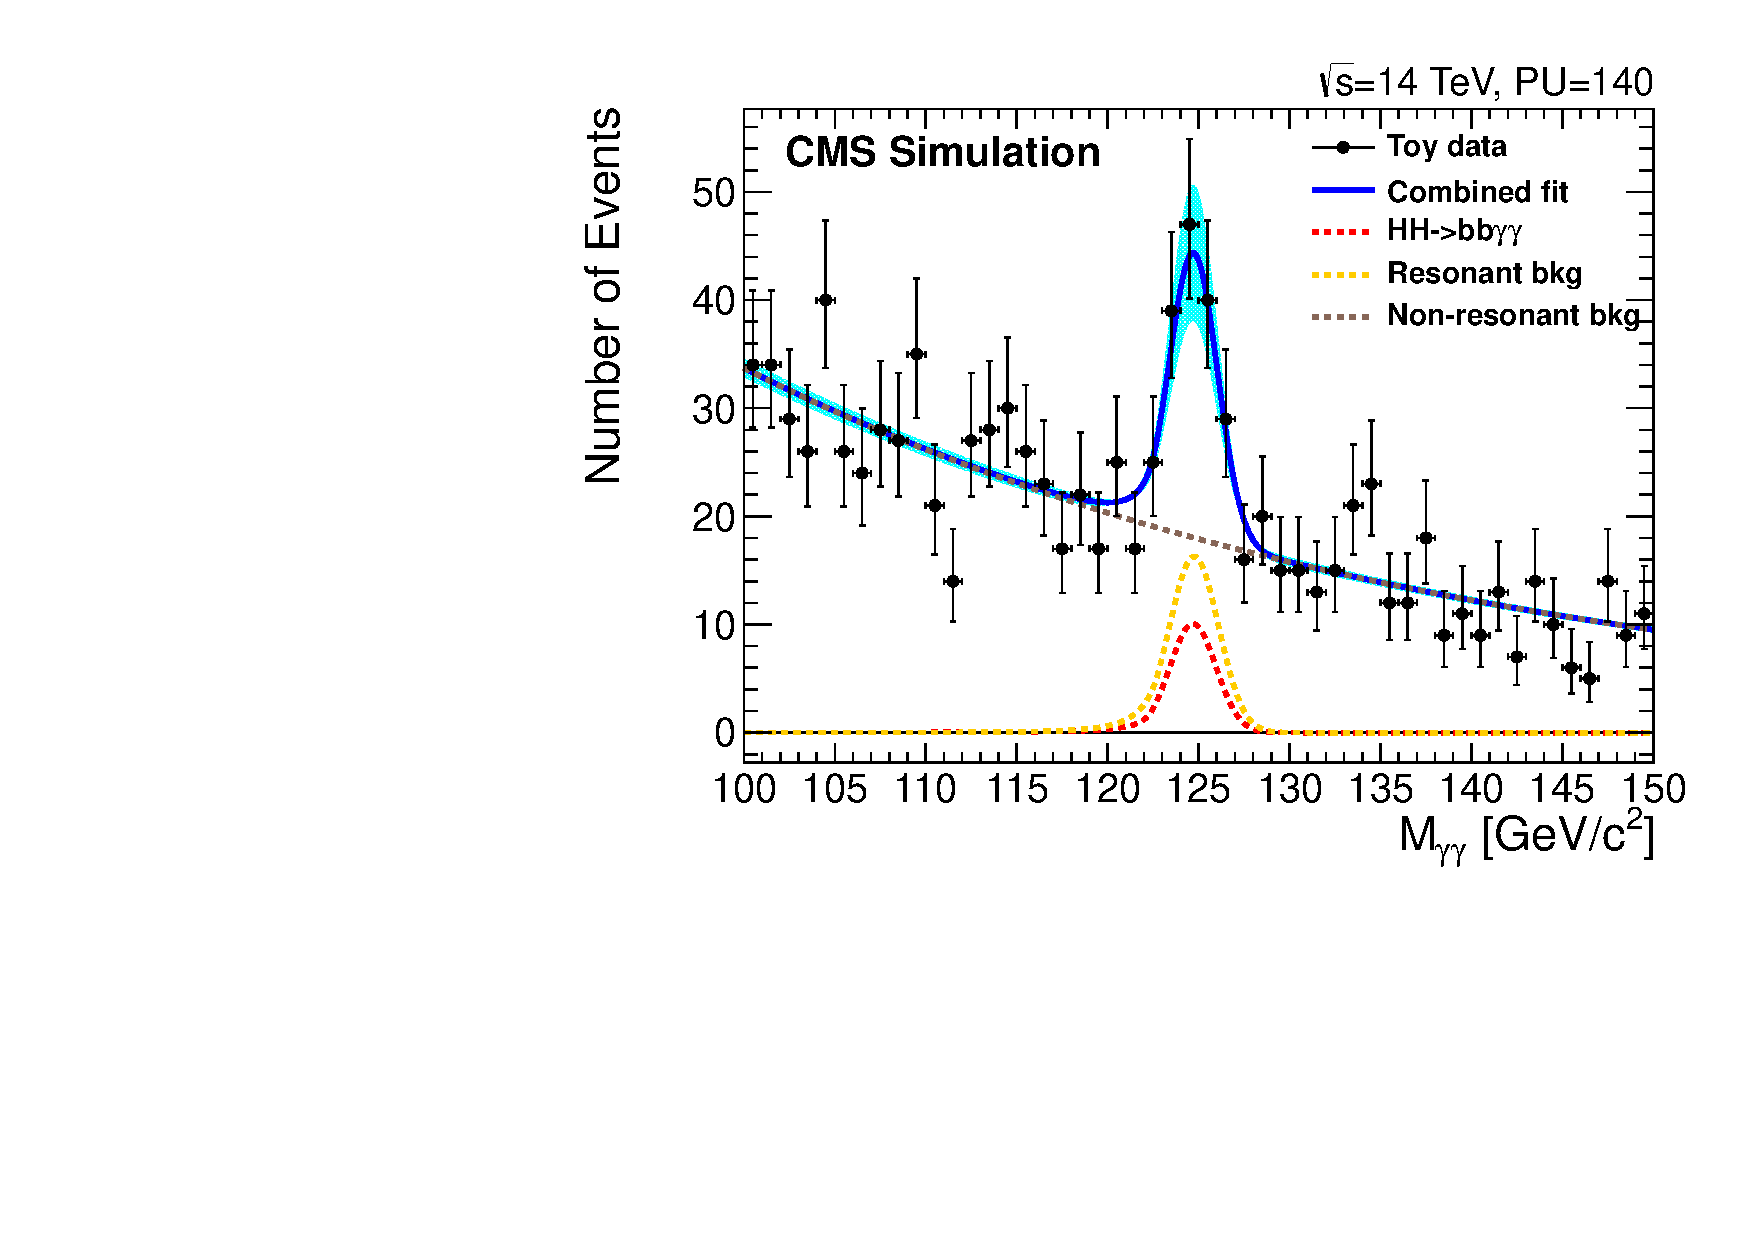
\includegraphics[width=0.8\textwidth]{figures_chapter6/hh_bbgg_mgg.pdf}
  \caption{Projection of a two dimensional fit on the di-photon mass for one representative
  toy experiment is shown. The signal, the resonant background, and the non-resonant background components are shown in 
  red, yellow, and gray, respectively.}
  \label{fig:twoDfullFitProjection}
\end{figure}
The statistical uncertainties dominate over the systematic uncertainties with $3000$~$\mathrm{fb}^{-1}$ of integrated luminosity. The systematic uncertainty in the non-resonant background modeling is evaluated by  performing toy MC experiments where the assumed non-resonant background model used is the product of an exponential and a fourth-degree polynomial fitted to the expected non-resonant background distribution, while an exponential function is used to perform the fit. This results in an
average bias of about $12\%$. The theoretical uncertainties in the Higgs boson pair production cross section coming from the missing higher order perturbative corrections, uncertainties in the $\alpha_{s}$ and the PDFs~\cite{Baglio:2012np} is about $11\%$. The systematic uncertainties in the jet and photon energy resolutions are negligible compared to the statistical uncertainty.

\subsection{Upgrade Scenarios}
\label{sec:scenarios}

It is critical to achieve a robust reconstruction of the detector objects at the HL-LHC pileup condition as discussed in Section 5.1. As the measurement is primarily limited by the number of selected signal candidate events, improving the object selection efficiency is very important to improve the results. To explore the effect of the object selection efficiencies and to provide a general goal for the detector upgrade, Figure~\ref{fig:PhotonEffImprovementScan} shows the sensitivity as a function of the relative improvement on the photon selection efficiency and the b-tagging efficiency, respectively, over the current performance estimate at the HL-LHC pileup conditions. It is seen that the measurement can be significantly improved with even a modest improvement in the photon candidate selection efficiency or b-tagging efficiency. 

\begin{figure}[h]
  \centering
  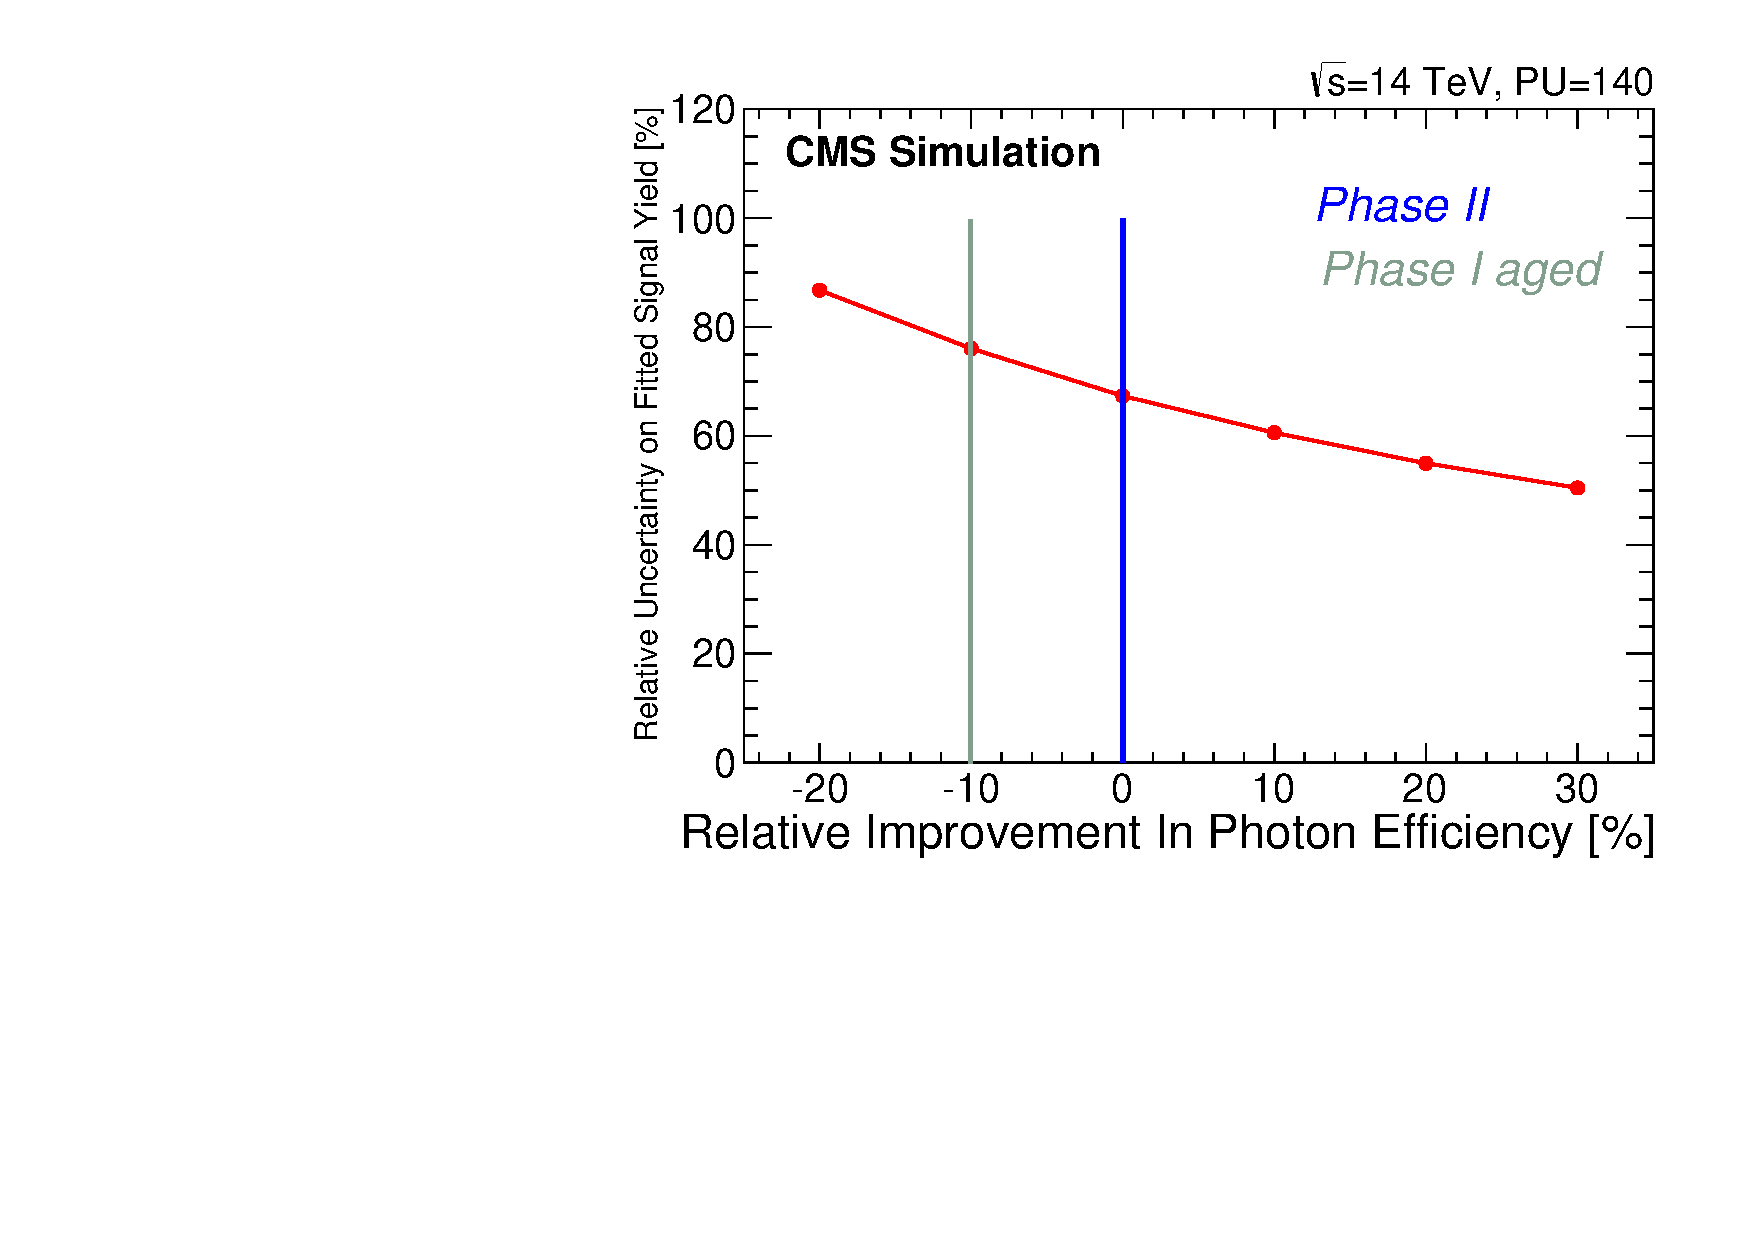
\includegraphics[width=0.49\textwidth]{figures_chapter6/XSUncertaintyVsPhotonEffRatio.pdf}
  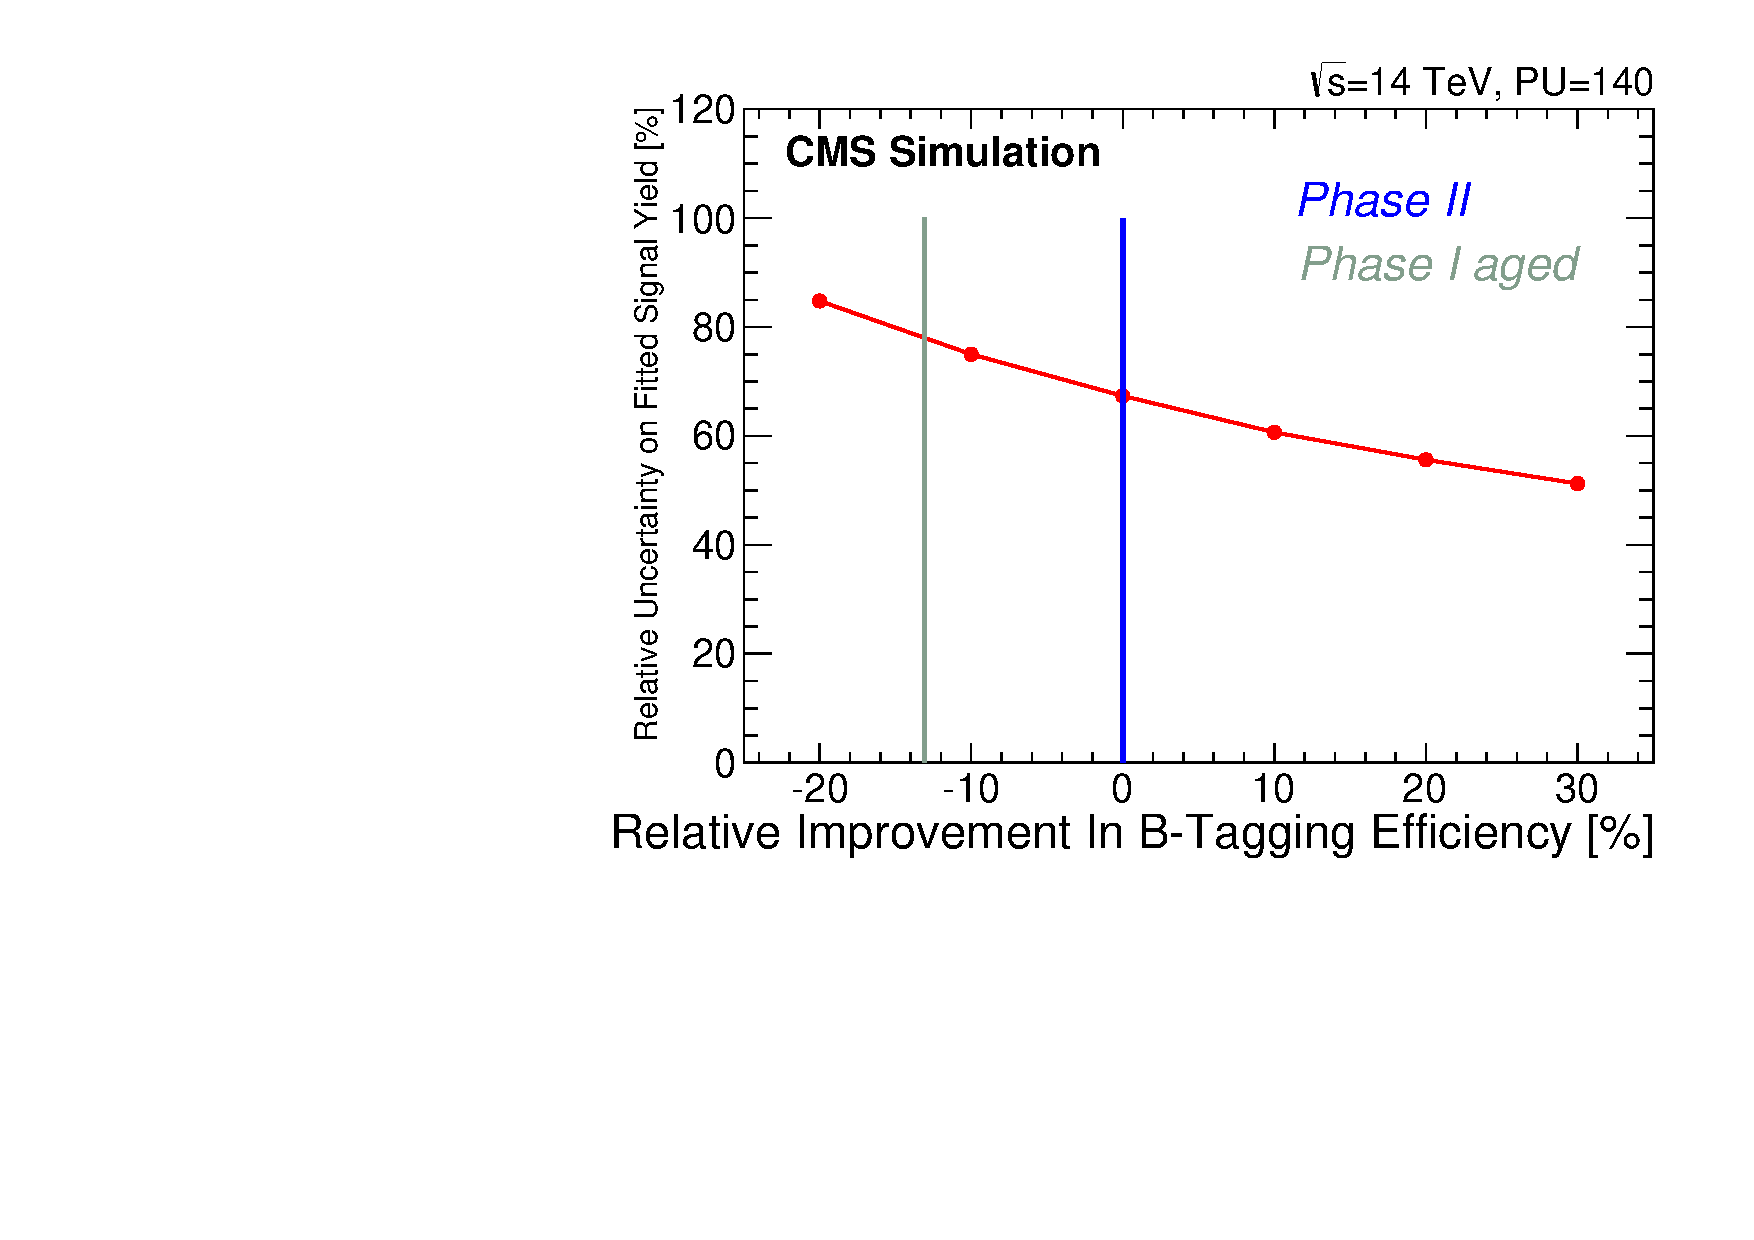
\includegraphics[width=0.49\textwidth]{figures_chapter6/XSUncertaintyVsBtagEffRatio.pdf}
  \caption{ The average expected relative uncertainty in the Higgs pair production cross section measurement as a function of the relative improvement in the photon (left) and b-tagging (right) selection efficiency with respect to the current performance estimate at the HL-LHC pileup conditions.}
  \label{fig:PhotonEffImprovementScan}
\end{figure}


Finally, the sensitivity of the result as a function of the total integrated luminosity (left) and the relative contribution of the non-resonant background contribution (right) is shown in Figure~\ref{fig:LumiScan}.

\begin{figure}[h]
  \centering
  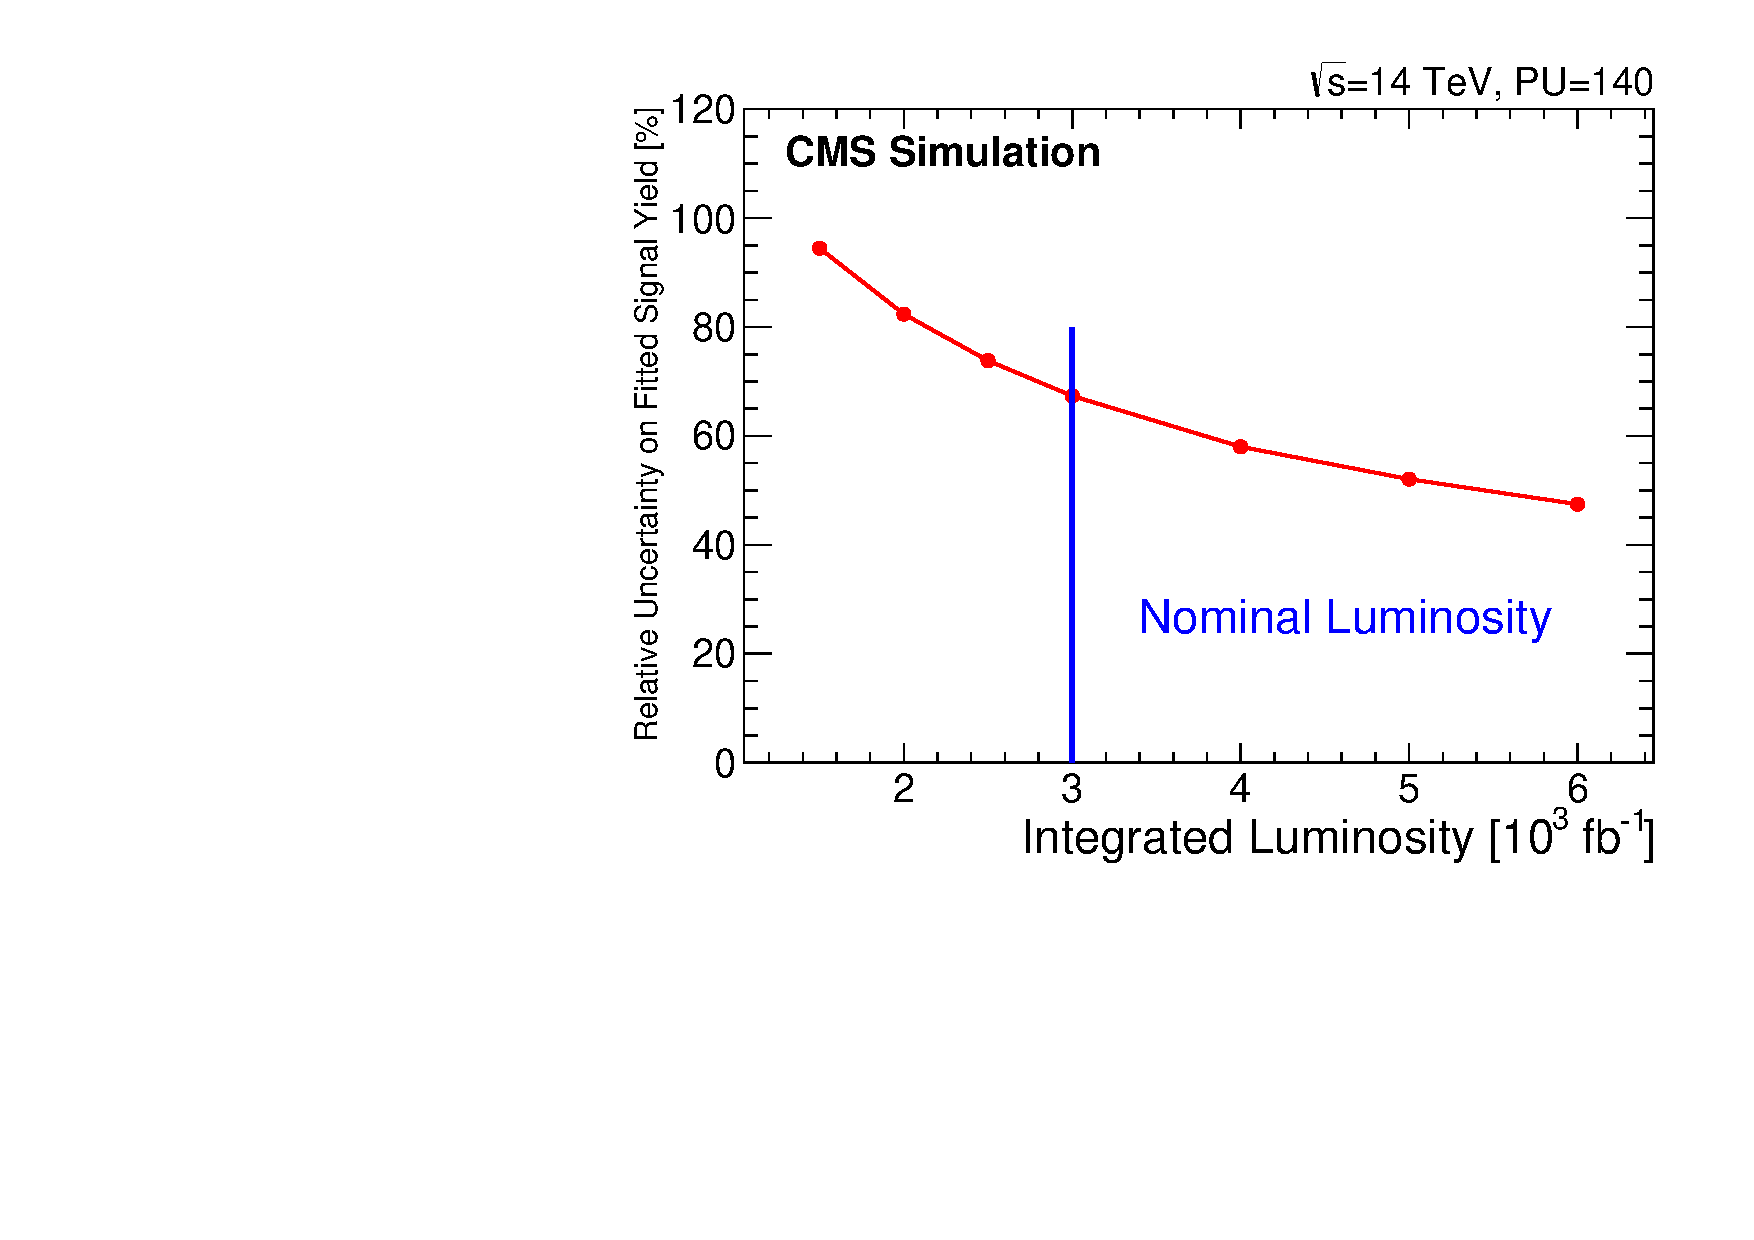
\includegraphics[width=0.48\textwidth]{figures_chapter6/XSUncertaintyVsLumi.pdf}
 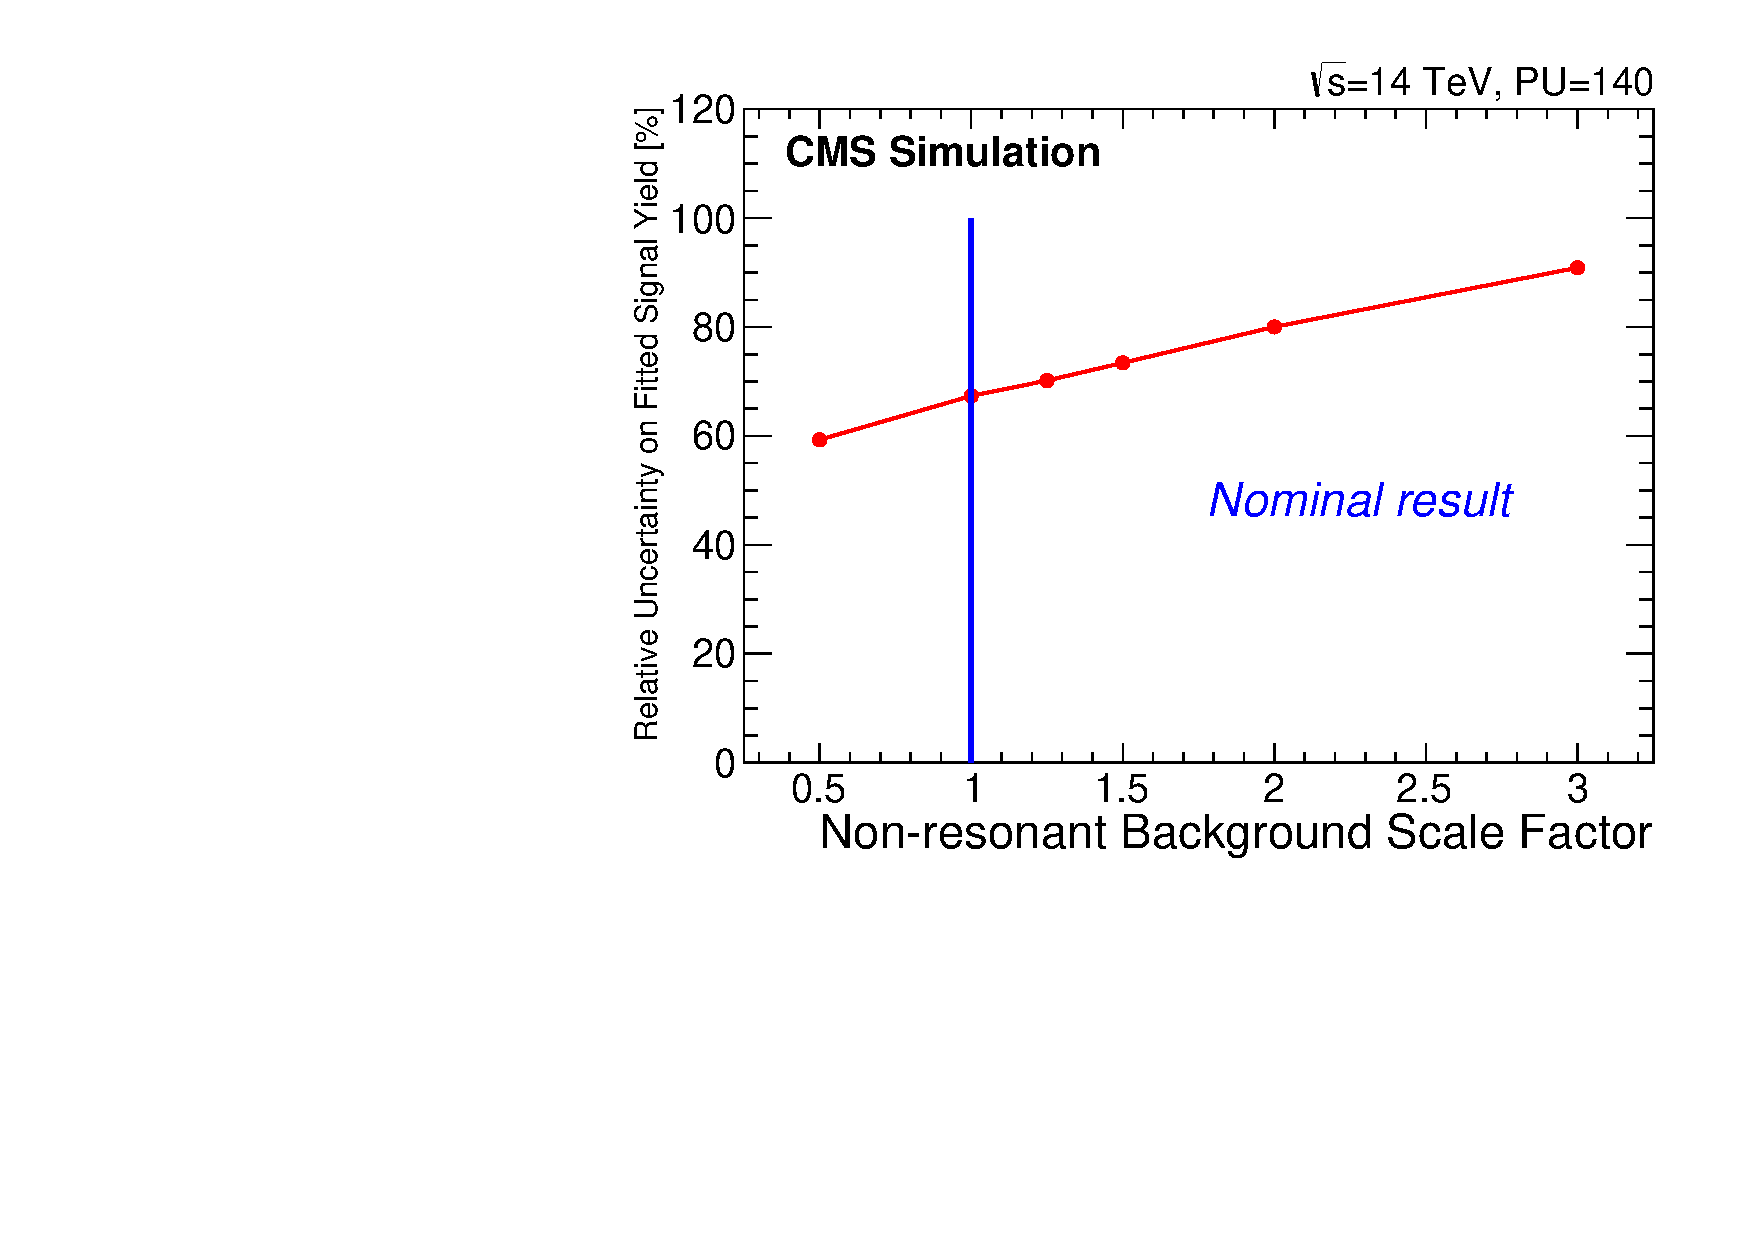
\includegraphics[width=0.48\textwidth]{figures_chapter6/XSUncertaintyVsNonResBkgScaleFactor.pdf} 
  \caption {The average expected relative uncertainty in the Higgs pair production cross section measurement is shown  as a function of the integrated luminosity (left) and the relative contribution of the non-resonant background.}
  \label{fig:LumiScan}
\end{figure}


\section{$bb\tau\tau$ Final State}

The signal events of interest contain two high $p_{T}$ taus and two high $p_{T}$ jets originating from b quarks. Di-tau final states $\tau_{\mu}\tau_{h}$ and $\tau_{h}\tau_{h}$ are considered. The jets are reconstructed using the anti-kt algorithm with a resolution parameter of $0.4$. A simple jet pileup identification is developed in Delphes using the track related and jet shape variables described in Section 3.5.2. The efficiency of the jet pileup identification is $0.95$ with a pileup jet rate of $0.20$. Without pileup mitigation the PF $\vec{E}_{T}^{miss}$ resolution is on average $50$~GeV with $140$ pileup interactions. With the PUPPI pileup mitigation the $\vec{E}_{T}^{miss}$ resolution in Delphes is reduced to about $25$~GeV.  The efficiency of selecting jets originating from b quarks and tau hadronic decays are parameterized in Delphes. To further reduce the background events with light jets mimicking the hadronic tau decays it is required that jets originating from hadronic tau decays contain an isolated track. With the upgraded \phasetwo detector and the $\tau_{h}$ selection described here, a selection efficiency of about $55\%$ is possible while keeping the mistag rates to be less than $0.5\%$. The working point used for the b-tagging has an average efficiency of $0.68$ with $0.1$ and $0.01$ mistag rates from the c-quarks and light quarks respectively.  The muon efficiencies and resolutions are parameterized in Delphes and efficiencies of about $95\%$ are assumed.

\subsection{Event Selection and Background Estimation}
Events are selected containing two b-tagged jets with $p_{T}>30$~GeV
and $|\eta|<2.4$, and two $\tau_{h}$ candidates with $p_{T}>60$~GeV, or $p_{T}>90$~GeV
for the leading $\tau_h$ candidate and $p_{T}>45$~GeV for sub-leading $\tau_h$ candidate, and
$|\eta|<2.1$ for the $\tau_{h}\tau_{h}$ di-tau final state, $p_{T}>30$~GeV
and $|\eta|<2.1$  for the $\tau_{h}$ and $p_{T}>30$~GeV and $|\eta|<2.5$
for the $\tau_{\mu}$ in $\tau_{\mu}\tau_{h}$ di-tau final states. 

The background samples are simulated using the techniques that were developed for the Snowmass 2013 Energy Frontier for the future hadron colliders~\cite{Avetisyan}. The existing generated samples were reconstructed using Delphes. A similar approach to the $bb\gamma\gamma$ analysis is adopted by producing a generator particle level $t\bar{t}$ sample and weighting the events by their corresponding efficiencies for selecting the constituent particles. The resolution effects of the detector are also taken into account. The main background is $t\bar{t}$ production with fully leptonic decays. Another source of large background is the Drell-Yan
production of a $Z$ boson decaying into a pair of tau leptons
produced in association with jets, where the light jets are mistagged as b-jets. The important single Higgs boson backgrounds are the $ZH$ and  $t\bar{t}H$ processes. The remaining backgrounds considered are the single top and $t\bar{t}$ produced in association with a vector boson, and di-boson processes.
The QCD multi-jet background is negligible in the signal region as verified by studying the LHC data available at $\sqrt{s} = 8$~TeV. 

\subsection {Signal Extraction}
 Selections are applied on the di-tau mass, $m_{\tau\tau}$, and the di-b-jet mass, $m_{bb}$, distributions to identify
the Higgs boson decays to tau and b pairs, respectively. The requirement for the $m_{bb}$ is $90$~GeV$<m_{bb}<130$~GeV, and
$110$~GeV$<m_{\tau\tau}<140$~GeV for the $m_{\tau\tau}$. The event selection is summarized in Table~\ref{tab:event_selection} 

\begin{table}[!ht]
\begin{center} 
\resizebox{\textwidth}{!}{
\begin{tabular}{|c|c|}
\hline
Event selection                                    \\ \hline
$\geq 2$ b-tagged jets with $p_{T}>30$~GeV, $|\eta|<2.4$ \\ \hline
$\tau_{h}\tau_{h}$ final state                     \\ 
$\geq 2$ isolated $\tau_{h}$-s with $p_{T}>60$~GeV or $p_{T}>90/45$~GeV, $|\eta|<2.1$  \\ \hline
$\tau_{\mu}\tau_{h}$ final state                     \\ 
An isolated $\tau_{h}$ with $p_{T}>30$~GeV, $|\eta|<2.1$ and an isolated $\tau_{\mu}$ with  $p_{T}>30$~GeV, $|\eta|<2.5$ \\ \hline 
 $90$~GeV$<m_{bb}<130$~GeV and $110$~GeV$<m_{\tau\tau}<140$~GeV \\ \hline
\end{tabular}
}
\caption{ Event selection summary for the bb$\tau\tau$ final state.}
\label{tab:event_selection}
\end{center}
\end{table}

A kinematic bounding variable, $m_{T2}$, is introduced to further
discriminate the dominant $t\bar{t}$ background from the Higgs boson pair signal~\cite{smt}. By construction, $m_{T2}$ is 
bounded above by the top quark mass for $t\bar{t}$ background events
while it is unbounded for di-Higgs boson signal events. For the
$\tau_{\mu}\tau_{h}$ final states a boosted decision tree (BDT) discriminant was trained to further exploit the boosted kinematics of the Higgs boson pair production. The input variables are the masses, transverse momenta, and $\Delta R$ distances of the di-tau, di-b-jet, and di-Higgs systems. The $m_{T2}$ variable is also included in the training.

Figure~\ref{fig:bdtout} shows the predicted distributions of the $m_{T2}$ variable (left) for the $\tau_{h}\tau_{h}$ final state and the BDT discriminant variable (right) for the $\tau_{h}\tau_{\mu}$ final state after the mass window requirements. Both variables provide good discrimination between the signal and background. As expected the $t\bar{t}$ background is bounded above by the top quark mass taking into account the detector resolution effects. Table~\ref{tab:hhsig} and Table~\ref{tab:mhsig} show the expected event yields with $3000 \mathrm{fb}^{-1}$ integrated luminosity at various stages of the event selection for the $\tau_{h}\tau_{h}$, and $\tau_{\mu}\tau_{h}$ final states, respectively. 

\begin{figure}[hbtp]
\begin{center}
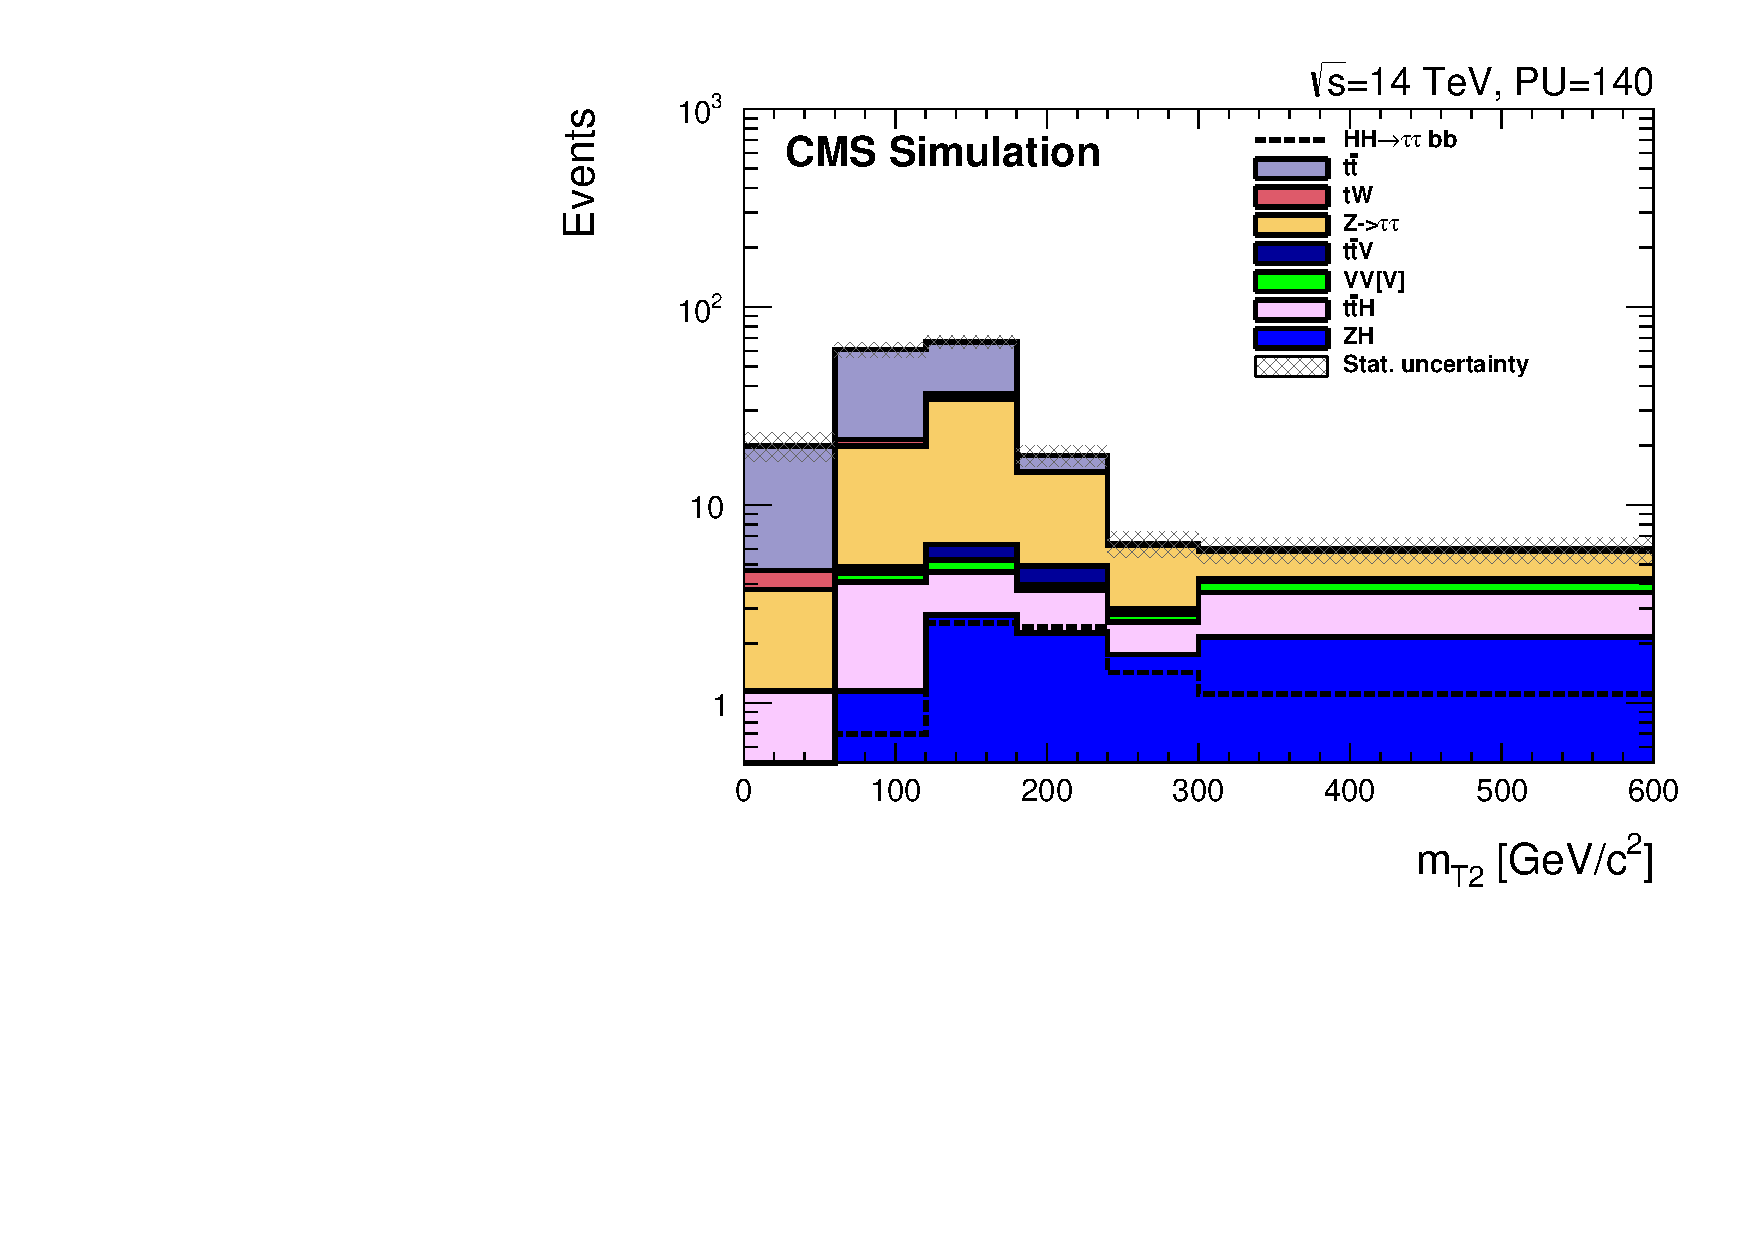
\includegraphics[width=0.49\textwidth]{figures_chapter6/thth_mt2.pdf}   
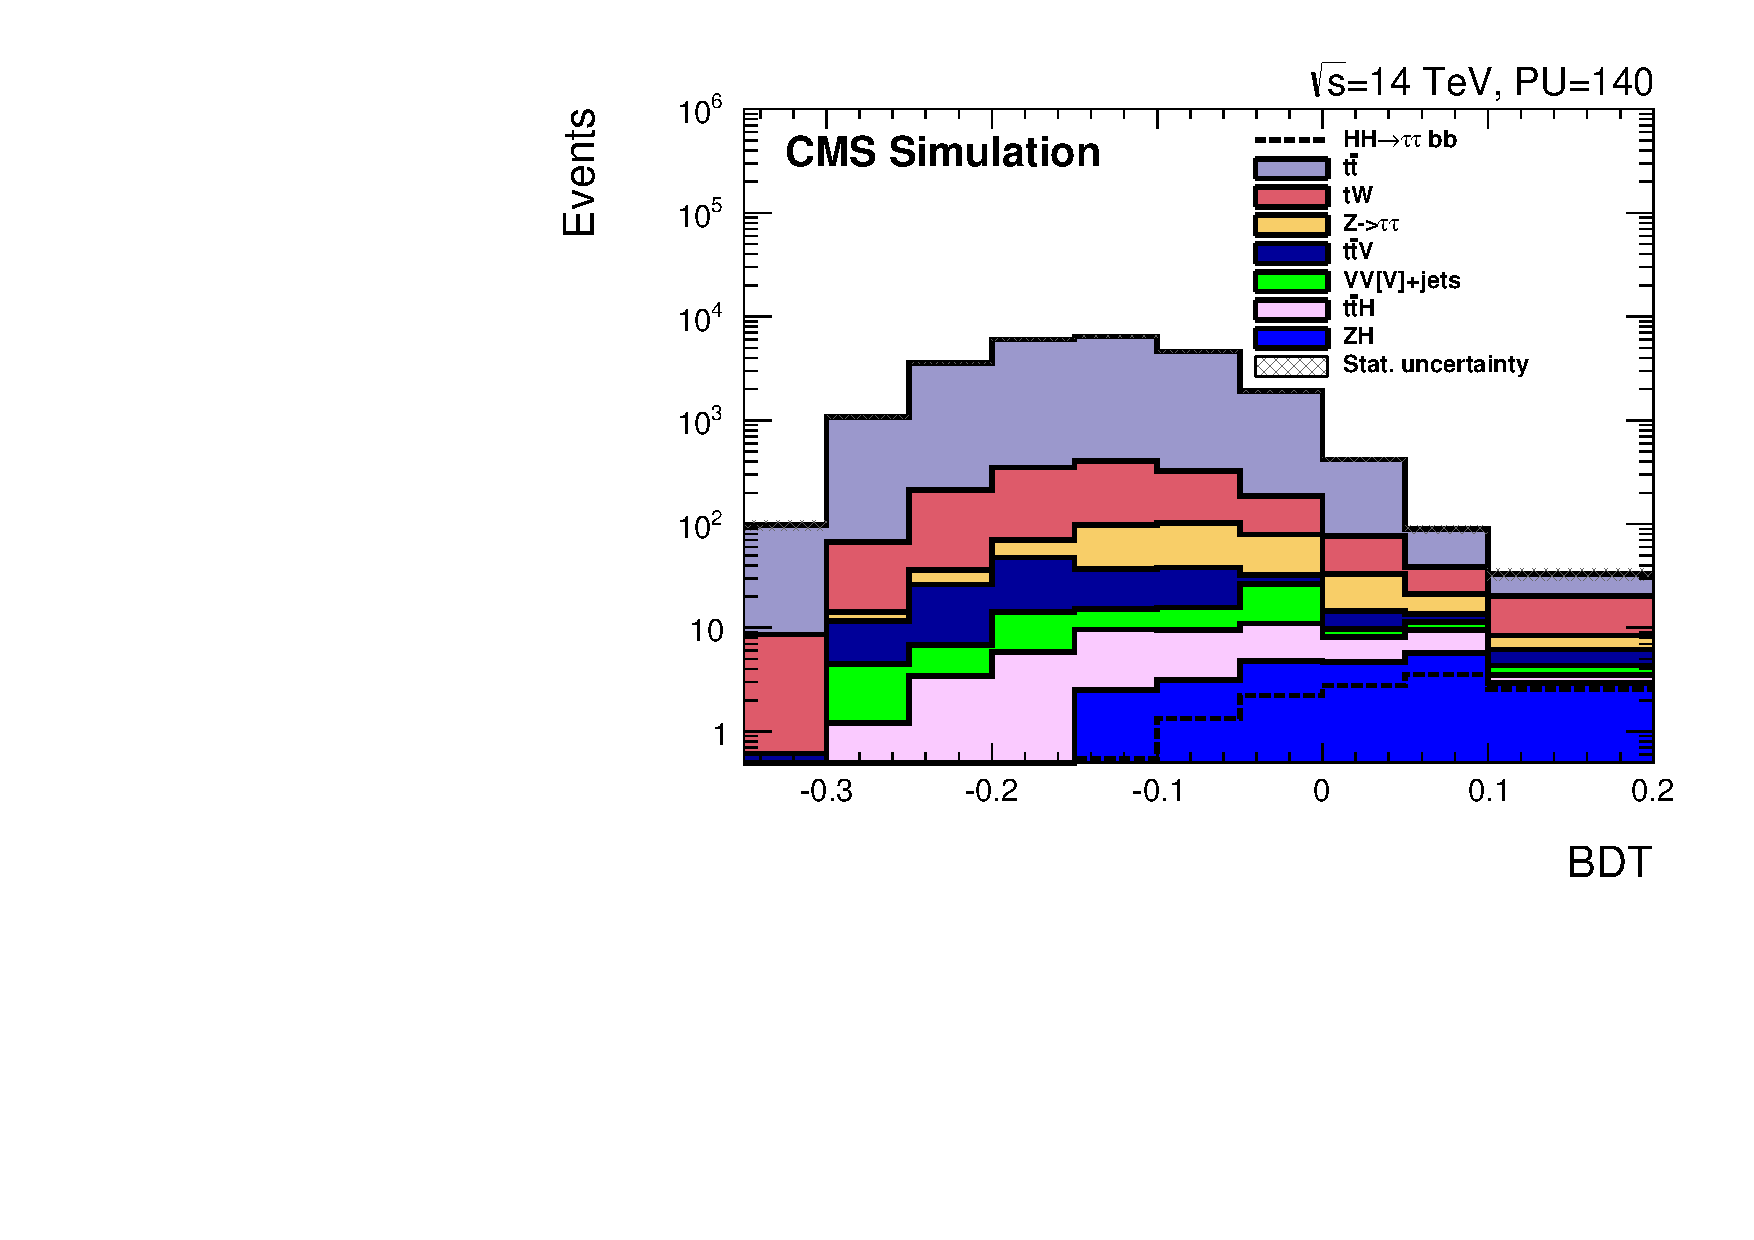
\includegraphics[width=0.49\textwidth]{figures_chapter6/tmth_bdt.pdf}
\caption{$m_{T2}$ (left) and BDT score (right) distributions in  the $\tau_{h}\tau_{h}$ and  $\tau_{\mu}\tau_{h}$ final states respectively. The yields are the expected SM contributions.}
\label{fig:bdtout}
\end{center}
\end{figure}

The expected significance for the Higgs boson pair production is $0.5$ and $0.7$ standard deviations for the $\tau_{\mu}\tau_{h}$ and $\tau_{h}\tau_{h}$ di-tau final states respectively. The combined expected significance is $0.9$ standard deviations. The resulting expected uncertainty in the cross section measurement is approximately $105\%$. Theoretical uncertainties in the Higgs boson production are
included in this result. Renormalization and factorization scale
uncertainties in the Higgs boson pari-production signal are $20\%$ for NNLO
calculation. The PDF uncertainty is $9\%$. The systematic uncertainty in
the luminosity is taken to be $2.6\%$. Energy scale uncertainties on jets, tau leptons, and missing energy are also included. A scale uncertainty of $2\%$ is assumed which is comparable to the corresponding uncertainty with the current CMS detector performance. The effect of the jet energy scale uncertainty in the result is about $5\%$.       

\begin{table}[!ht]
\begin{center} 
\begin{tabular}{|c|c|c|c|c|}
\hline
Selection  & $HH$ & $ZH$ & $t\bar{t}H$ & $Z\rightarrow \tau\tau$  \\  \hline
Baseline selection & $23.6\pm0.5$ & $104.7\pm3.5$ & $204.6\pm5.8$ & $479.3\pm7.7$  \\
Mass windows  & $8.3\pm0.3$ & $10.1\pm1.0$ & $9.8\pm1.3$ & $60.3\pm3.3$ \\ 
Signal  & $4.9\pm0.2$ & $6.2\pm0.8$ &  $3.8\pm0.8$ & $14.7\pm1.6$ \\ \hline
\end{tabular}

\vspace{2mm}

\begin{tabular}{|c|c|c|c|c|}
\hline
Selection   & $t\bar{t}$ & $tW$ & $t\bar{t}V$ & $VV(V)$  \\  \hline
Baseline selection & $7662\pm69$ & $734.4\pm19.4$ & $189.4\pm10.0$ & $128.9\pm16.7$  \\
Mass windows  & $88.4\pm7.5$ & $4.8\pm1.6$ & $2.7\pm0.9$ & $2.1\pm0.7$ \\ 
Signal  & $3.2\pm1.4$ & $0.1\pm0.1$ & $1.3\pm0.7$ & $1.0\pm0.5$ \\ \hline
\end{tabular}

\caption{ The expected signal yields at $3000$~$\mathrm{fb}^{-1}$ of integrated luminosity are shown at various stages of the  selection in the $\tau_{h}\tau_{h}$ channel. A loose mass window cut is applied on the $t\bar{t}$ sample at the  generation level. For the signal selection stage the $m_{T2}$ is required to be greater than $180$~GeV. The full $m_{T2}$ distribution is used for the signal extraction.}
\label{tab:hhsig}
\end{center}
\end{table}


\begin{table}[!ht]
\begin{center} 
\begin{tabular}{|c|c|c|c|c|}
\hline
Selection  & $HH$ & $ZH$ & $t\bar{t}H$ & $Z\rightarrow \tau\tau$  \\  \hline 
Baseline selection & $39.2\pm0.6$ & $213.7\pm4.7$ & $1175.8\pm12.9$ & $3711.7\pm34.1$  \\
Mass window  & $13.1\pm0.4$ & $24.4\pm1.5$ & $37.7\pm2.3$ & $234.5\pm8.6$  \\ 
Signal  & $6.1\pm0.3$ & $8.6\pm0.9$ & $4.5\pm0.8$ & $9.7\pm1.7$ \\ \hline
\end{tabular}

\vspace{2mm}
\resizebox{\textwidth}{!}{
\begin{tabular}{|c|c|c|c|c|}
\hline
Selection  & $t\bar{t}$ & $tW$ & $t\bar{t}V$ & $VV(V)$  \\  \hline
Baseline selection & $(3.84\pm0.00)\times10^{5}$ & $(3.72\pm0.00)\times10^{4}$ & $4154\pm39$ & $1418\pm90$ \\
Mass window   & $(2.3\pm0.0)\times10^{4}$ & $1232\pm33$ & $119.4\pm7.4$ & $49.6\pm2.3$   \\ 
Signal   & $63.5\pm7.3$ & $29.2\pm4.8$ & $3.9\pm1.3$  & $2.7\pm0.7$ \\ \hline
\end{tabular}
}
\caption{ The expected signal yields at $3000$~$\mathrm{fb}^{-1}$ of integrated luminosity are shown at various stages of the selection in the $\tau_{\mu}\tau_{h}$ channel. A loose mass window cut is applied on the $t\bar{t}$ sample at the generation level. For the signal selection stage we require the BDT variable to be greater than $0.05$. The full BDT distribution is used for the signal extraction.}
\label{tab:mhsig}
\end{center}
\end{table}

\subsection{Trigger Performance}
The performance of the trigger system is crucial to achieve the result
described above, in particular the capability to trigger on charged
particles at L1 trigger. For the $\tau_{h}\tau_{h}$ final state, the
di-tau trigger has an offline threshold of $56$~GeV on both tau legs,
and the single tau trigger threshold is $88$~GeV for the L1 trigger  of the \phasetwo upgraded detector~\cite{Butler:2020886}.  These thresholds are significantly higher without the inclusion of tracks in the L1 trigger (track trigger), $95$~GeV on both tau legs for the di-tau trigger and $138$~GeV for the single tau trigger. Considering these less performant thresholds, the signal and background yields are reduced by about a factor of
two. For the $\tau_{\mu}\tau_{h}$ final state the situation is similar. The single-muon trigger
threshold is $18$~GeV with the track trigger and $50$~GeV without the track
trigger. The thresholds for the muon-tau trigger legs are significantly
higher as well. Again, the signal and background yields are reduced by a factor of two
by requiring $50$~GeV cut on the $p_T$ of the muon and $\tau_h$.
Thus, in both final states the effect of the trigger performance on the sensitivity of this analysis is significant. The overall sensitivity is
reduced by 40\%, the equivalent of  using only half of 3000~fb$^{-1}$.

\section{Results and Summary}
A combination of the  $bb\gamma\gamma$ and $bb\tau\tau$ results is performed by using a simultaneous fit to the generated pseudo-data. The expected uncertainty in the signal yield is approximately $54\%$. The combined expected significance is $1.9$ standard deviations. The studies are performed assuming the operational conditions of the HL-LHC, with an integrated luminosity of 3000~$\mathrm{fb}^{-1}$, and the upgraded CMS detector.  The benefits of the CMS \phasetwo upgrades to meet the challenges presented by the high luminosity environment are emphasized. Further improvements of the sensitivity are possible by using more sophisticated reconstruction and analysis techniques. Additional Higgs boson pair production boson production and decay modes remain unexplored. Among these the bbbb final state promises the largest potential for improvement.
